\chapter*{Introduction générale}
\label{chap:intro}
\addcontentsline{toc}{chapter}{\nameref{chap:intro}}

\section{Contexte et motivations}
\label{sec:intro:contexte}
Une décision judiciaire peut être définie soit comme  le résultat rendu par les juges à l'issue d'un procès, soit comme un document décrivant une affaire judiciaire. Un tel document rapporte, notamment,  les faits, les procédures judiciaires antérieures, le verdict des juges, et les explications associées. Dans cette thèse, nous désignons par \og décision \fg{} le document, et par  \og résultat\fg{} une conclusion ou réponse des juges. Une jurisprudence
%\footnote{\url{http://www.toupie.org/Dictionnaire/Jurisprudence.htm}} 
est un ensemble de décisions rendues par les tribunaux. Elle représente la manière dont ces derniers interprètent les lois pour résoudre un problème juridique donné (type de contentieux). Les juristes doivent alors collecter des décisions traitant de situations similaires, les sélectionner, et les analyser afin de mener, par exemple, des recherches empiriques en droit \citep{ancel2003expulsion, jeandidier2006pensions}. Les avocats exploitent aussi les décisions passées pour anticiper les résultats des juges. Ils peuvent ainsi mieux conseiller leurs clients sur le risque judiciaire que ces derniers encourent, et sur la stratégie à adopter pour faire accepter leurs demandes et faire rejeter celles de leurs adversaires. Cette activité de collecte et d'analyse, centrale pour de nombreux métiers du droit, est généralement effectuée manuellement. Elle est par conséquent sujette à plusieurs difficultés liées à l'accès et à l'exhaustivité des documents traités même lors de l'étude d'une question spécifique. Il faut notamment souligner ici que les documents sont dispersés dans les nombreux tribunaux, et que les procédures administratives ne facilitent pas toujours leur accès du fait de la nécessité de préserver la confidentialité des parties. En effet, les décisions n'étant pas \og anonymisées \fg{} la plupart du temps, elles restent alors inaccessibles aux juristes qui en font la demande. Un certain nombre de documents sont néanmoins accessibles sur internet grâce à des sites de publication de données ouvertes gouvernementales\footnote{Données ouvertes gouvernementales: \hyperlink{http://data.gouv.fr}{data.gouv.fr} en France, \hyperlink{https://www.judiciary.uk}{judiciary.uk} en Grande-Bretagne, \hyperlink{http://www.scotusblog.com/}{scotusblog.com} aux Etats-Unis, et \hyperlink{https://www.scc-csc.ca/}{scc-csc.ca} au Canada.}. Ces sites publient régulièrement des décisions récemment prononcées. 

\begin{figure}[!htb]
	\centering
	\begin{subfigure}[t]{\textwidth}
		\centering
		\fbox{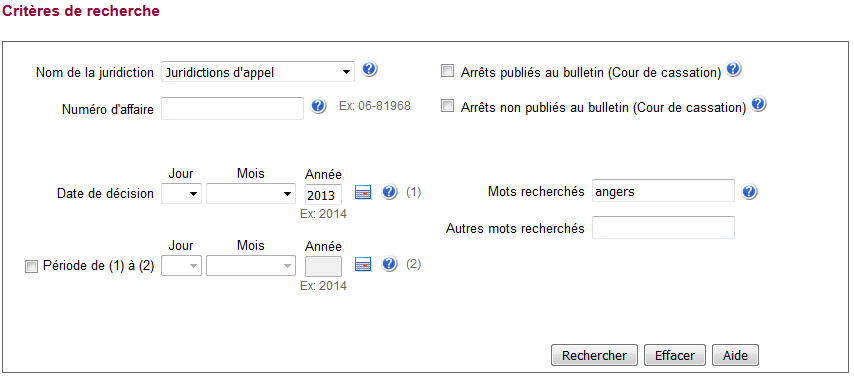
\includegraphics[width=\textwidth]{legifrance.PNG}}
		\caption{Formulaire de Légifrance}
	\end{subfigure}%

	\begin{subfigure}[t]{0.75\textwidth}
		\centering
		\fbox{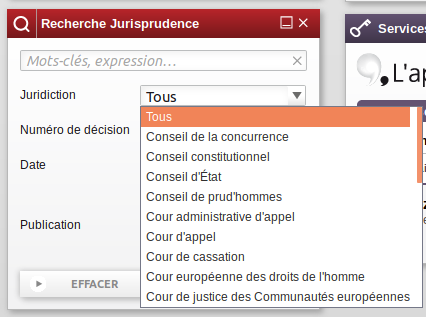
\includegraphics[width=\textwidth]{dalloz.png}}
		\caption{Formulaire de Dalloz}
	\end{subfigure}
% 	\begin{subfigure}[t]{0.56\textwidth}
% 		\centering
% 		\fbox{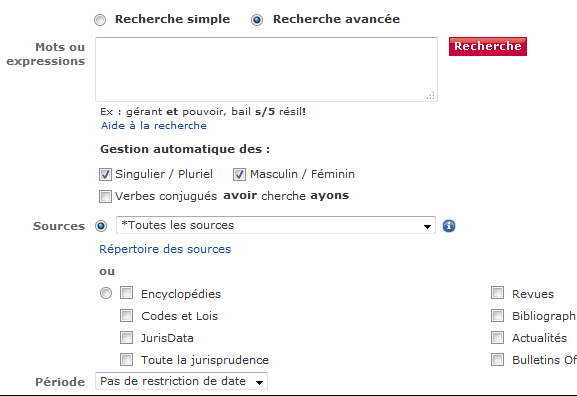
\includegraphics[width=\textwidth]{lexisnexis.png}}
% 		\caption{Formulaire de LexisNexis}
% 	\end{subfigure}%
	\caption{Exemples de critères des moteurs de recherche juridique}\label{fig:intro:juriSearchForm}
\end{figure}

Il existe aussi des moteurs de recherche juridiques qui permettent de retrouver des décisions intéressantes. Cependant, qu'ils soient payants (LexisNexis\footnote{\url{https://www.lexisnexis.fr/}}, Dalloz\footnote{\url{http://www.dalloz.fr}}, Lamyline\footnote{\url{http://lamyline.lamy.fr}},...) ou gratuits (CanLII\footnote{\url{https://www.canlii.org}}, Légifrance\footnote{\url{https://www.legifrance.gouv.fr}}, ...), les critères de recherche offerts par leurs moteurs de recherche limitent grandement la pertinence des résultats pouvant être obtenus. En effet, il ne s'agit en général que de combinaisons de mots-clés et autres méta-données (date, type de juridiction, ...), ou d'expressions régulières, comme l'illustre la \figureref{fig:intro:juriSearchForm}. La manipulation de tels critères est difficile pour constituer des échantillons pertinents suivant une sémantique souhaitée tels que l'ensemble des décisions traitant d'une catégorie de demande ou d'une circonstance factuelle donnée. 

\begin{table}[!htb]
 	\small
 	\begin{center}
 		\begin{tabular}{|l|l|l|l|l|l|}
 			\hline
 			\textbf{Justice}	& \textbf{2013}  & \textbf{2014}  & \textbf{2015}  & \textbf{2016}  & \textbf{2017}  \\ \hline
 			civile   & 2 761 554 & 2 618 374 & 2 674 878 & 2 630 085 & 2 609 394 \\ \hline
 			pénale   & 1 303 469 & 1 203 339 & 1 206 477 & 1 200 575 & 1 180 949 \\ \hline
 			administrative & 221 882 & 230 477 & 228 876 & 231 909 & 242 882 \\ \hline
 		\end{tabular}
 		
 		\textit{\scriptsize{\textbf{Source}: \url{http://www.justice.gouv.fr/statistiques-10054/chiffres-cles-de-la-justice-10303/}}}  
 	\end{center}
 	\caption{Nombre de décisions prononcées en France par an de 2013 à 2017}\label{tab:intro:nbdecisionstats}
 \end{table}
Plus de 4 millions de décisions sont prononcées en France chaque année d'après les chiffres du ministère français de la justice (\tableref{tab:intro:nbdecisionstats}). Dans ce contexte, l'analyse manuelle ne peut être limitée qu'à une infime proportion de documents disponibles.
En effet, au regard de la croissance rapide du nombre de décisions, même une étude sur une question très précise nécessite la constitution d'un large corpus de décisions pertinentes. Par ailleurs, il peut s'avérer très pénible de les lire pour en identifier les données d'intérêt. Les documents sont très souvent longs et complexes dans leur style de rédaction. Par exemple, Certaines phrases comprennent plusieurs clauses discutant d'aspects différents (\figureref{fig:intro:multiclauses}). On y retrouve aussi des références à des jugements antérieurs (\figureref{fig:intro:referencejugementanterieur}).
\begin{figure}[!htb]
\fvset{gobble=2, numbers=left, fontsize=\footnotesize}
\begin{Verbatim}[firstnumber=69]
  Exposant subir un trouble anormal de voisinage pour être privée d'une vue sur la 
  mer dont elle disposait auparavant, ce en raison de l'absence de taille de haies 
  implantées à proximité de son jardin privatif, elle a attrait devant le juge des 
  référés du tribunal de grande instance de Marseille, le syndicat des 
  copropriétaires LES CATALANS (ci-après désigné : le syndicat des copropriétaires) 
  , et son syndic recherché personnellement, le Cabinet L., à l'effet, au visa de 
  l'article 809 du code de procédure civile d'obtenir leur condamnation sous 
  astreinte de 200 euros par jour de retard à tailler les haies qui bouchent sa 
  vue et la condamnation personnelle du Cabinet L. à lui régler une provision de 
  2.000 euros à valoir sur dommages et intérêts, outre 1.500 euros sur le 
  fondement des dispositions de l'article 700 du code de procédure civile.
\end{Verbatim}
\scriptsize{\textit{\textbf{Source}: extrait de la décision R.G. 15/10226 de la Cour d'Appel d'Aix-en-Provence du 2 Juin 2016}}
  \caption{Exemple de phrases composée de plusieurs clauses dont une demande de condamnation sous astreinte, une autre de dommages et intérêts pour trouble anormal de voisinage, et une dernière de dommages et intérêts sur l'article 700 du code de procédure civile.}
  \label{fig:intro:multiclauses}
\end{figure}


\begin{figure}[!htb]
\fvset{gobble=2, numbers=left, fontsize=\footnotesize}
\begin{Verbatim}[firstnumber=73]
    Vu le jugement du tribunal de grande instance de Versailles du 5 décembre 2013 
    qui a :
    - rejeté la demande de démolition de la construction litigieuse,
\end{Verbatim}
\begin{Verbatim}[firstnumber=118, stepnumber=2]
    ...
    SUR CE LA COUR,
\end{Verbatim}
\begin{Verbatim}[firstnumber=277, stepnumber=2]
    ...  
    PAR CES MOTIFS, 
    ...
\end{Verbatim}
\begin{Verbatim}[firstnumber=281]
    Confirme le jugement en toutes ses dispositions à l'exception de celle relative 
    au montant des dommages et intérêts ...
\end{Verbatim}
\footnotesize{\textit{\textbf{Source}: extrait de la décision R.G. 14/01640 de la Cour d'Appel de Versaille du 7 Avril 2016}}
  \caption{Exemple de référence à un jugement antérieur dans une décision d'appel.}
  \label{fig:intro:referencejugementanterieur}
\end{figure}
Il est évident qu'une automatisation du traitement des corpus de décisions s'impose pour répondre aux diverses difficultés d'accès, de volumétrie, et de complexité liées à la compréhension des décisions. Une telle automatisation ferait gagner du temps aux juristes lors de tâches d'analyse métier préalables à leur raisonnement d'experts, tout en leur fournissant une vue exhaustive de la jurisprudence. D'autre part, \citet{cretin2014justicecomplexe} fait remarquer que la justice est complexe dans son organisation (\figureref{orgjusticefrance}) et son fonctionnement, et que son langage est peu compréhensible. Il est donc presque impossible pour les profanes en droit d'estimer leurs droits et le risque judiciaire qu'ils encourent dans leur quotidien sans consulter un initié du droit. L'exigence pour le profane étant l'exacte pertinence des ressources, leur accessibilité, et l'intuitivité du processus de leur exploitation \citep{narazenko2017legalnlpintro}, l'automatisation de l'analyse de la jurisprudence pourrait ainsi améliorer l'accessibilité du droit dans d'indénombrables situations. Par exemple, en comparant le montant qu'on peut espérer d'une juridiction et le coût d'un procès, on peut plus aisément se décider entre un arrangement à l'amiable et la poursuite du litige en justice \citep{langlaischappe2009ecoresolutionlitige}. Le traitement automatique de la jurisprudence constituerait alors une aide précieuse non seulement pour les professionnels du droit, mais aussi pour les particuliers et entreprises tous soucieux de voir l'issue de leur affaire leur être favorable.  

\begin{figure}[!htb]
	\centering 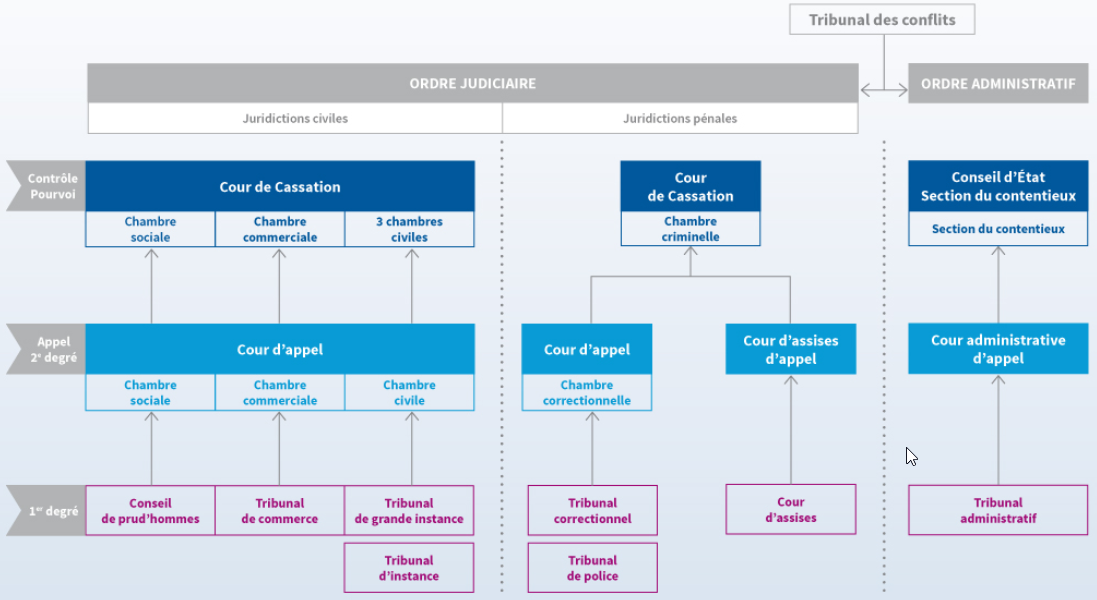
\includegraphics[angle=90,width=0.65\textwidth]{organisation_justice_francaise_grand.png}
	
	\textit{\scriptsize{\textbf{Source}: \url{http://www.justice.gouv.fr/organisation-de-la-justice-10031/}}}  
	\caption{Organisation des institutions judiciaires françaises} \label{orgjusticefrance}
\end{figure}

\section{Objectifs}
%\textcolor{red}{Description d'une approche traditionnelle, exemple d'études, difficultés de ces études}
 Ce mémoire propose des approches pour automatiser l'extraction de connaissances judiciaires à partir des décisions françaises. Le but est de faciliter la structuration et l'analyse descriptive et prédictive de corpus de décisions de justice en adressant les difficultés de l'approche traditionnelle d'analyse de contentieux. L'étude de la jurisprudence pour un contentieux donnée consiste à \citep{ancel2003expulsion} :
 \begin{enumerate}
 	\item \textbf{Choisir un échantillon représentatif}: Des décisions sont collectionnées suivant des contraintes définies:  période précise, couverture géographique, types d'affaires, etc.
 	\item \textbf{Sélectionner les décisions}: élimination des décisions qui ne correspondent pas au type de demande d'intérêt.
 	\item \textbf{Élaborer la grille d'analyse}: Un modèle de grille est créé et permet d'enregistrer les informations potentiellement importantes. Chaque ligne de la grille correspond à une demande, et les colonnes font référence aux différents types d'informations qu'il est possible d'extraire sur une demande. Ces variables vont de la procédure suivie, aux solutions proposées, en passant par la nature de l'affaire. Les champs à remplir ne sont pas connus à l'avance ; ce n'est généralement qu'au cours de la lecture des décisions que l'on distingue les informations pertinentes pour l'étude.
 	\item \textbf{L'analyse des décisions et l'interprétation des informations}: Les informations retrouvées dans les décisions sont saisies dans la grille, et des calculs statistiques sont effectués par la suite.
 \end{enumerate}
 
\citet{ancel2003expulsion} évoque principalement le problème de la différence entre l'état capté de la jurisprudence et son état présent. En effet, les longs délais de travail sont caractéristiques de ces études. L'étude de son équipe portait sur les décisions d'expulsion d'occupants sans droit ni titre. La saisie des informations à elle seule a duré 9 mois.  De plus, il est difficile d'observer l'évolution des pratiques judiciaires dans le temps et leur différence entre les villes du fait de la faible taille de l'échantillon choisi. Par exemple, \citet{jeandidier2006pensions} n'ont analysé que 399 dossiers d'affaires de pension alimentaire correspondant aux audiences s'étalant de fin 1999 à fin 2000 d'un seul tribunal de grande instance. L'équipe de \citet{ancel2003expulsion} n'a quant à elle analysé que 3865 décisions sélectionnées parmi 5656 décisions rendues du 1$^\text{er}$  juillet au 31 décembre 2001. 
 
La problématique de notre étude est \og \textbf{comment donner accès à l'analyse automatique de la sémantique d'un corpus jurisprudentiel pour comprendre la prise de décision des juges?} \fg{}. La complexité de cette analyse s'explique notamment par l'interprétation subjective des règles juridiques, l'application non déterministe de la loi, et la technicité du langage judiciaire. Cette problématique intéresse des entreprises telles que LexisNexis, et plusieurs startups  telles que Predictice\footnote{\url{http://predictice.com}} et CASE LAW ANALYTICS\footnote{\url{http://caselawanalytics.com}}. Afin d'y répondre, nous nous intéressons aux concepts d'informations mentionnées dans les décisions, au centre desquels se trouvent les demandes des parties (prétentions) sur lesquelles portent les conclusions rendues. Ainsi, l'analyse sémantique d'un corpus jurisprudentiel vise l'identification de connaissances sur les demandes (Figure \ref{fig:intro:demande-central}).
 \begin{figure}[!htb]
 	\centering
 	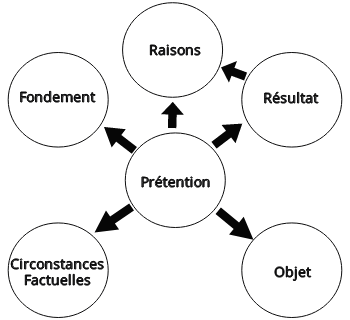
\includegraphics[scale=0.7]{demande-central.png}
 	
 	\scriptsize{\textit{Sens des flèches: l'extrémité est l'information sur l'origine.}}
 	\caption{La demande au centre de la compréhension des décisions}
 	\label{fig:intro:demande-central}
 \end{figure} 

Une demande peut être caractérisée par :
 \begin{itemize}
 	\item l'objet qui a été demandé (par ex. dommages et intérêts) quantifié par un quantum ;
	\item le résultat associé qui est décrit par une polarité (\og accepte \fg{} ou \og rejette \fg{}), souvent lié à un quantum accordé, par exemple 5000 euros de dommages et intérêts ou 2 mois d'emprisonnement;
	\item le fondement ou la norme juridique qui est la règle qui légitime la prétention ou le résultat;	
	\item les circonstances factuelles caractérisant les types d'affaires ;
	\item les divers arguments apportés par les parties pour justifier leurs requêtes  (raisons des demandes).
	\item les motivations des solutions des juges (raisons des résultats)
 \end{itemize}

Ces concepts descriptifs d'une demande couvrent l'essentiel de l'information pertinente pour les experts. 

Cette thèse s'inscrit dans un projet qui vise, entre autres, à automatiser l'extraction de l'ensemble de ces informations et de les structurer afin d'enrichir une base de connaissances sur la jurisprudence française. Une telle base permettrait notamment de mener des études sur différents critères comme la juridiction, le type de demande, ou encore les circonstances des litiges. Elle aurait aussi naturellement une importance certaine pour la définition de modèles prédictifs par exemple pour la prédiction des types de demandes à formuler et la prédiction de la solutions des juges. 

%Le projet comprend deux phases principales : une phase d'indexation des connaissances de la masse des décisions, suivie d'une analyse prédictive. La phase d'indexation doit déjà permettre de réaliser automatiquement, de manière exhaustive, des analyses descriptives. Ces dernières consistent, par exemple, à comparer le nombre d'acceptations à la fréquence des rejets. Par conséquent, le système doit apprendre à reconnaître dans les décisions, les informations pertinentes sur les prétention et résultats associés. La phase d'analyse prédictive consiste à regrouper des paquets de décisions similaires (même résultat sur la même prétention dans les circonstances similaires), pour découvrir les facteurs influençant le sens du résultat (par ex. le fait que \og le revenu de l'époux soit le plus élevé du foyer\fg{} encourage les juges à accorder la pension alimentaire à l'épouse). En effet, c'est la connaissance de ces facteurs circonstanciels qui permet à l'expert de pouvoir anticiper les décisions judiciaires.

 La chaîne de traitement à mettre en \oe uvre se compose de quatre étapes principales qui s'enchaînent comme le présente la Figure \ref{fig:intro:pipeline-globale}. Notre étude s'intéresse donc aux problématiques liées à la constitution de la base de connaissance et à son exploitation dans un contexte d'analyses descriptives. Celles-ci sont décrites dans la suite.

\begin{figure}[!htb]
	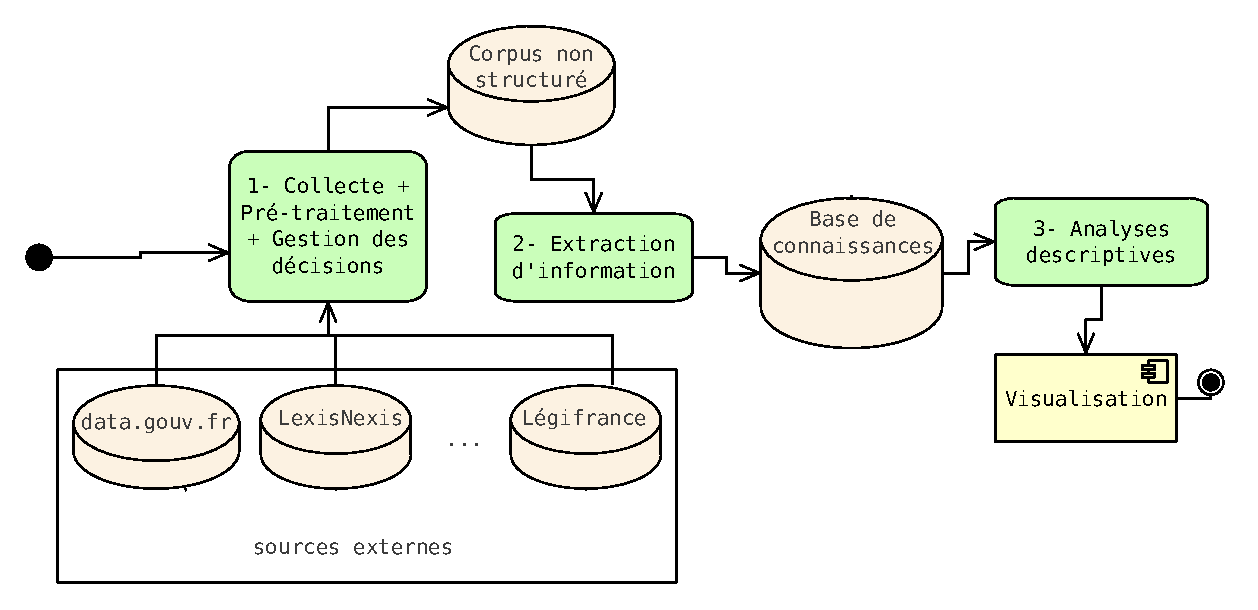
\includegraphics[width=\textwidth]{pipeline-cassandra.pdf}
	\caption{Chaîne d'analyse du corpus jurisprudentiel à mettre en \oe uvre} \label{fig:intro:pipeline-globale}
\end{figure} 


\subsection{Collecte, gestion et pré-traitement des documents}
Il est nécessaire de trouver des moyens pour collecter le maximum de documents bruts non-structurés, les pré-traiter, et organiser leur gestion afin de les indexer pour faciliter leur traitement. Les décisions de cours d'appel de justice civile sont les plus accessibles à partir des moteurs de recherche juridique (LexisNexis, Dalloz, LamyLine, Legifrance, etc.) et de la grande base de données JuriCa. Cependant, l'accès à ces décisions est généralement payant, et le nombre de documents simultanément téléchargeables est très faible sur les sites payants (généralement 10 à 20 décisions au maximum à la fois). De plus, le nombre de téléchargements par jour est limité. La base JuriCa est la plus grosse base de décisions de cours d'appel en France. Elle est gérée par la Cour de cassation. L'accès à cette base est offert par le Service de Documentation, des Etudes et du Rapport\footnote{\url{https://www.courdecassation.fr/institution_1/composition_56/etudes_rapport_28.html}} (SDER). L'accès est payant pour les professionnels et gratuit pour les universités et centres de recherche en partenariat avec le SDER. Légifrance, le moteur de recherche du ministère de la justice, fournit quant à lui un accès public et gratuit à un nombre considérable de documents. Les décisions y sont identifiées à l'aide de numéros consécutifs et accessibles à partir d'un service web. Ce dernier a l'avantage de proposer des décisions de tous les ordres et de tous les degrés. Cependant, les décisions des juridictions du premier degré (appelées jugements) restent plus rares sur internet et principalement disponibles auprès des tribunaux.  La disponibilité des décisions du second degré ou d'appel (appelées arrêts) en justice civile est l'une des raisons pour lesquelles notre étude s'est portée sur celles-ci.

%Les décisions existent sous divers formats PDF, DOC, DOCX, RTF, TXT, XML, etc. Il arrive parfois qu'un fichier téléchargé comprenne plusieurs décisions (sur LexisNexis par exemple). Nous avons par conséquent préféré convertir tous les documents au format plein texte pour homogénéiser les traitements. Par ailleurs, les décisions sont collectées à partir de diverses sources pouvant contenir des documents identiques. Il se pose donc un problème d'identification unique des décisions pour éviter des redondances. Pour cela, nous avons défini une convention de nommage des fichiers. Ce dernier repose sur 3 informations: le type de juridiction (tribunal, cour d'appel, ...), la ville, et le numéro R.G. (registre général) qui est l'identifiant unique de la décision au sein de la juridiction. Par exemple, le numéro \og CAREN1606137 \fg{} identifie la décision de numéro R.G. \og 16/06137 \fg{} de la cour d'appel (\og CA \fg{}) de la ville de Rennes (\og REN \fg{}). Ces 3 informations sont présentes dans les premières lignes de la décision, et sont facilement identifiables à l'aide d'une routine à base de règles simples. D'autre part, certains moteurs de recherche ne fournissent souvent qu'un résumé au lieu du contenu original des décisions. Il est important de supprimer ces fichiers du corpus.

\subsection{Extraction de connaissances}
\label{subsec:intro:ie}
%Les problématiques d'extraction de connaissances constituent la pierre angulaire de cette thèse car les informations sur les demandes, les parties, les juges, les juridictions et les faits conditionnent la qualité des prévisions du sens du résultat pour un type de demandes considéré.  
La difficulté d'extraire de telles informations découlent de l'état non-structuré des documents, et de la complexité et la spécificité du langage employé. L'extraction des connaissances nécessite de mettre en \oe uvre des techniques de fouille de textes adaptées à la nature des éléments à identifier. Nous avons ainsi abordé l'annotation des références de l'affaire (juridiction, ville, participants, juges, date, numéro R.G., normes citées, ...), l'extraction des demandes et résultats correspondants, et l'identification des circonstances factuelles.

Les métadonnées de référence sont des segments de texte qu'on peut directement localiser dans le document. Elles sont donc semblables aux entités nommées dont la reconnaissance est une problématique intensivement étudiée en traitement automatique du langage naturel \citep{yadav2018surveyNeuralNER} dans plusieurs travaux et compétitions, aussi bien pour des entités communes \citep{tjong2003introCoNLL,grishman1996muc6}, que pour des entités spécifiques à un domaine \citep{kim2004bioNer, persson2012nbbioner,hanisch2005prominer}, et dans diverses langues \citep{li2018wcpbioner,alfred2014malayner,amarappa2015kannada}. 

Le problème d'identification des demandes consiste à reconnaître, dans la décision analysée, l'objet, le fondement, le quantum demandé, le sens du résultat correspondant, et le quantum accordé de chaque prétention. La demande s'apparente donc aux entités structurées telles que les évènements \cite{ace2005event} qui sont décrits par un type, un terme-clé, des participants, un temps, une polarité.

Le problème d'identification des circonstances factuelles consiste à constituer des regroupements de décisions mentionnant une certaine catégorie de demande (objet+fondement). Le but est, comme indiqué précédemment, de repérer les différentes situations dans lesquelles cette catégorie de demande est formulée. Chacun des groupes représente donc une situation particulière partagée par les membres du groupe mais bien distinctes de celles reflétées par les autres groupes. Ce problème évoque des problématiques de similarité entre textes, de catégorisation non-supervisée (\textit{clustering}), et de \og modélisation thématique \fg{} (\textit{topic modeling}). 

A l'issue du processus d'extraction, les données extraites sont destinées à enrichir progressivement une base de connaissances. La structuration des données au sein d'une base facilite les diverses analyses automatiques applicables aux décisions et demandes judiciaires. 

\subsection{Analyse descriptive}
L'analyse descriptive exploite l'ensemble des connaissances extraites et organisées pour répondre aux diverses questions que l'on pourrait se poser sur l'application de la loi. Il est intéressant par exemple de comparer les fréquences de résultats positifs et négatifs pour une catégorie de prétention donnée dans une situation précise. Les quanta extraits servent à visualiser les différences entre les montants accordés et réclamés. D'autres analyses plus complexes permettraient d'étudier l'évolution dans le temps et les différences dans l'espace de l'opinion des juges.


\section{Méthodologie}
\label{sec:intro:methodologie}
Les tâches sont définies par le métier.
Comme illustrées précédemment (\ref{subsec:intro:ie}), les problématiques propres aux textes juridiques trouvent généralement des analogies avec les problèmes d'analyse de données textuelles (\textit{text mining}). Ainsi, les méthodes issues de ce domaine sont applicables aux textes juridiques. Cependant, quelques adaptations sont généralement nécessaires pour obtenir des résultats de bonne qualité hors des domaines pour lesquels ces approches ont été développées \citep{Waltl2016lexia}. De plus, la recherche en fouille de textes est souvent réalisée sur des échantillons qui ne reflètent pas toujours la complexité des données réelles. Effectuant l'une des premières études d'analyse sémantique des décisions françaises, nous avons axé notre travail sur le rapprochement des problèmes liés à l'analyse des décisions jurisprudentielles de ceux généralement traités en analyse de textes. Il s'agit ensuite d'établir des protocoles d'évaluation et d'annotation manuelle de données. Selon les problématiques identifiées et les protocoles d'évaluations définis, des méthodes adaptées ont été proposées et expérimentées sur les données réelles annotées manuellement par un expert juriste.

\section{Résultats}
\label{sec:intro:résultats}
Une chaîne de traitement pour le sectionnement et l'annotation des méta-données est proposée. Premièrement, le sectionnement a pour but d'organiser l'extraction des informations qui sont réparties dans des sections selon leur nature. L'applicabilité de deux modèles probabilistes, les champs aléatoires conditionnels ou CRF (\textit{conditional random fields}) et les modèles cachés de Markov ou HMM (\textit{hidden Markov Model}), est étudiée en considérant plusieurs aspects de la conception des systèmes d'extraction d'entités nommées.  

Par la suite, nous proposons une méthode d'extraction des demandes et des résultats en fonction des catégories présentes dans la décision. L'approche consiste en effet à identifier dans un premier temps les catégories (objet+fondement) présentes par classification supervisée. Un vocabulaire d'expression des demandes et résultats est exploité pour identifier les passages. Puis à l'aide de termes propres à chacune des catégories identifiées, les trois attributs (quantum demandé, sens du résultat, quantum accordé) des paires demande-résultat sont reconnus. 

Par ailleurs, nous analysons l'extraction du sens du résultat par classification binaire des documents. L'objectif est de s'affranchir de l'identification préalable de l'expression des demandes et résultats. En effet, les décisions comprenant des demandes d'une catégorie donnée semblent ne contenir, dans une forte proportion, qu'une seule demande. %Nous pensons qu'il n'est par conséquent pas nécessaire d'identifier l'expression de cette dernière pour en déterminer le sens. 
A partir d'une représentation adéquate du contenu de la décision, il est possible de classer cette dernière à l'aide d'un modèle de classification supervisée de documents.

L'identification des circonstances factuelles, quant à elle, est modélisée comme une tâche de regroupement non supervisé de documents. Nous proposons dans ce cas une méthode d'apprentissage d'une distance entre textes, à l'aide d'un algorithme de régression. La métrique apprise est utilisée dans l'algorithme des \og K-moyennes \fg{} (\textit{k-means}) \citep{forgey1965kmeans} et celui des \og K-medoïdes \fg{} (\textit{k-medoids}) \citep{kaufman1987kmedoids}, et comparée à d'autres distances établies en recherche d'information.

\section{Structure de la thèse}
\label{sec:intro:organisation}

La thèse est organisée en 6 chapitres. Le chapitre \ref{chap:literature} positionne nos travaux par rapport à ceux qui ont été réalisés précédemment sur des problématiques d'analyse automatique de décisions de justice. Le chapitre \ref{chap:structuration} présente les architectures et modèles proposés pour la structuration des décisions et la reconnaissance des entités juridiques ; il discute notamment des différents résultats empiriques obtenus par application des modèles CRF et HMM. Ensuite, le chapitre \ref{chap:quanta} détaille le problème  d'extraction des demandes, puis présente notre méthode et les résultats obtenus. Le chapitre \ref{chap:sensresultat} traite de l'identification du sens du résultat par classification directe des décisions, cela en comparant différents algorithmes de classification et de représentations des textes. Le chapitre \ref{chap:similarite} discute de l'usage de l'apprentissage proposé d'une distance qui est comparée à d'autres distances pour la découverte des circonstances factuelles. Enfin, le chapitre \ref{chap:demo} présente des résultats de scénarios d'analyses descriptives pour illustrer l'exploitation potentielle de nos propositions sur un corpus de grande taille. 
